%%% Plantilla creada para Proyecto de Investigación
%%% Instituto TecnolÓgico Superior de Escarcega
%%% ANTONIO MORA NAVARRO
%%% Ver 1.0, 30 Mayo 2017
\documentclass[a4paper,10pt]{report} 

\usepackage[utf8]{inputenc}
\usepackage[spanish]{babel}
\usepackage{amsmath}
\usepackage{amsfonts}
\usepackage{amssymb} 

\usepackage{graphicx} 
\usepackage{hyperref} 
\usepackage{wrapfig}
\usepackage{enumitem}
\usepackage{fancyhdr}
\usepackage{float}
\usepackage{eurosym}
\usepackage{color}
\usepackage{titling}
\usepackage{lipsum}
\usepackage{tocbibind}


\usepackage[left=3cm,right=3cm,top=3cm,bottom=4cm]{geometry}


\pagestyle{fancy}

 
%%% Para las cabeceras
\newcommand{\hsp}{\hspace{20pt}}
\newcommand{\HRule}{\rule{\linewidth}{0.5mm}}
\headheight=50pt
%%% 
\newcommand{\vacio}{\textcolor{white}{hola}}

%%% Para que las ecuaciones se numeren
%%% con el número de sección y el de ecuación.
\renewcommand{\theequation}{\thesection.\arabic{equation}}


% Color azul para algunos 
% textos de la portada
\definecolor{azulportada}{cmyk}{0.5,0.7,1,0.1}

%%%% Azul para textos de headings
\definecolor{azulinterior}{cmyk}{0.5,1,0,0.1}

%%%%%%%%%%%%%%%%%%%%%%%%%%%%%%%%
%%%%%% Datos del proyecto %%%%%%
%%%%%%%%%%%%%%%%%%%%%%%%%%%%%%%%
%%%TÍTULO
%%% Escribirlo en minúsculas, el programa
%%% lo pondrá en mayúsculas en la portada.
\title{Disminución de los tiempos en el registro de un cliente en un hotel de Escárcega, Campeche a través de la implementación de un software de registro.}
%%%% AUTOR
\author{ANTONIO MORA NAVARRO}
%%%%%%%%%%%%%%%%
%%%%%% DIRECTOR DEL TRABAJO
%%%%%%% Cambiar el nombre siguiente
\newcommand{\director}{MC. Manuel Arturo Suarez Amendola }
%%%%%%%%%%%%%%%

%%%%%%%%%%%%%%%%%%%%%
%%%%%%%%%%%%%%%%%%%%
\begin{document}

%%%%%%%%%%%%%%%%%%%%%%%%%%%%%%%
%%%%%%%%%%%%%%%%%%%%%%%%%%%%%%%
\begin{titlepage} %%%%% Aquí no hay que tocar nada.
	%%%% Las siguientes instrucciones generarán automáticamente
	%%%% la portada de tu proyecto.
	%%% Cambio de la estructura de esta página
\newgeometry{left=0.6cm,top=1.3cm,bottom=1.2cm}

\fbox{\parbox[c]{18.5cm}{
\begin{center}
\vspace{1.5cm}
{\fontfamily{phv}\fontsize{20}{6}\selectfont{Instituto Tecnológico Superior de Escárcega}}\\
[1em]
{\fontfamily{phv}\fontsize{15}{5}\selectfont{Ingeniería En Sistemas Computacionales}}\\
[1em]
{\fontfamily{phv}\fontsize{18}{5}\selectfont{INFORME DE INVESTIGACIÓN}}\\
[2.6cm]
% Autor del trabajo de investigación
\textcolor{azulportada}{\fontfamily{phv}\fontsize{16}{5}\selectfont{\theauthor}}\\
[1cm]
% Título del trabajo
\textcolor{azulportada}
{\fontfamily{phv}\fontsize{30}{5}\selectfont{\textsc{\thetitle}}}\\
%{\Huge\textbf{\thetitle}}\\
[1cm]

\includegraphics[width=8cm]{logoitse.png}
\\[2cm]
{\fontfamily{phv}\fontsize{16}{5}\selectfont{Trabajo dirigido por}}\\
[0.5cm]
{\fontfamily{phv}\fontsize{16}{5}\selectfont{\director}}\\
[2cm]
{\fontfamily{phv}\fontsize{16}{5}\selectfont{curso Febrero - Julio 2017}}\\
[4cm]
\end{center}
}}
 
 \restoregeometry
 %%%% Volvemos a la estructura de la página normal

\end{titlepage}

%%%%%%%%%%%%%%%%%%%%%%%%%%%%%%

{%\Large

\newpage

%%%Encabezamiento y pie de página
%%% También se genera automáticamente
%%% Mejor no tocarlo mucho.
\renewcommand{\headrulewidth}{0.5pt}
\fancyhead[R]{
	\textcolor{azulinterior}{\fontfamily{phv}\fontsize{14}{4}\selectfont{\textbf{\thetitle}}}\\
\textcolor{azulportada}{\fontfamily{phv}\fontsize{10}{3}\selectfont{Taller de Investigación II -- curso Febrero - Julio 2017}}\\
{\fontfamily{phv}\fontsize{10}{3}\selectfont{\theauthor}}}
\fancyhead[L]{\vacio}

\renewcommand{\footrulewidth}{0.5pt}
\fancyfoot[L]{\footnotesize Instituto Tecnológico Superior de Escárcega --- curso Febrero - Julio2017}
\fancyfoot[C]{\vacio}
\fancyfoot[R]{\footnotesize Página \thepage}


%%%%%%%%%%%%%%%%%%%%




\newpage

%%% En esta página va el índice,
%%% pero no hay que hacer nada porque 
%%% se generará automáticamente.

\tableofcontents

\newpage



\section{\textbf{Introducción}}

En esta investigacion se pondra en evidencia las ventajas de los sistemas informaticos en
areas de trabajo, en este caso se buscará disminuir los tiempos en que un recepcionista de un 
Hotel de la región realiza el registro de un cliente implementando en si herramientas adecuadas para poder llevar a cabo una automatización del proceso de captura de los datos de registro de un cliente.
Se aplicaran encuestas para saber la opinion de los clientes al implementar programas de computo para llevar a cabo su solicitud de ingreso al hotel.
Asi como una guia de observacion para monitorear sus actitudes de ellos al momento del registro, y despues de esto.
Se implementara un programa de registro version beta para llevar a cabo una comparación al sistema de registro que actualmente cuenta el Hotel Akimpech, dando a conocer sus ventajas y desventajas de su aplicacion al local.
%

}
\

\

\

\

\section{Planteamiento del Problema}

El problema se presenta en los proceso de reserva, registro y facturación del huésped. Todo sucede cuando el posible huésped llama al hotel y se le toman los datos personales necesarios para validar la reserva. Este se guarda en un formato de papel y es archivado en un sección en donde se encuentran todas las reservas realizadas por que el sistema actual es incapaz de guardarlo, El proceso de registro se ejecuta de la siguiente manera; se ejecutan los datos del huésped y se confirma la reserva, pero como el sistema presenta dificulta para guardar dicha información, cuando este se cierra esta información desaparece, trayendo como consecuencia la perdida del cliente, por que cuando este llega al hotel al no aparecer la reservación se disgusta por que la habitación aparece ocupada por otra persona. Otra dificultad que se presenta en la facturación es que el sistema no registra el consumo que hace el cliente por tanto este proceso es llevado manualmente, muchas veces este registro no se hace adecuadamente lo que conlleva a que cuando el cliente pide su factura para cancelar no existe un registro detallado de lo que ha consumido y el cliente tiene que informar lo consumido durante su estadía. En esta situación se corre el riesgo de que el cliente de una información errada y el hotel registren perdidas por falta de registro oportuno de la información.


\section{Metodología}
Investigación Descriptiva: Es el tipo de investigación en que se pueden describir las características o situaciones que se presentan dentro de la empresa y se analizan factores e indicadores que pueden afectar el objeto de estudio. (Elaboración del plan de evaluación de desempeño al personal del Hotel Akimpech.) 

\

Investigación Propositiva: El estudio es propositivo porque comprende la elaboración de un programa de evaluación de admistracion basado en el desarrollo de competencia para mejorar la efectividad laboral del Hotel Akimpech de la Ciudad de Escarcega, Campeche que se presentará como propuesta con el fin de contribuir a la solución de la problemática existente.

\ 

\subsection{Caracterización o tipo del diseño de investigación: }
\  
· Pre experimental: Se realizara una comparación de registros de los clientes por parte del recepcionista, utilizando los metodos de registro utilizados actualmente en el hotel en comparacion del software de registro.

\section{Bitacora de actividades}
\begin{table}[H]
\centering
\begin{tabular}{|p{6cm}|p{2cm}|p{6cm}|}
\hline
Actividad & Fecha & Observaciones \\
\hline \hline
Delimitar nuestro tema de investigacion & 22-febrero-2017 & Definimos nuestro Tema de Investigación y nuestra Pregunta para que nuestro proyecto no fuese muy extenso en el momento de ponerlo en marcha. \\
\hline
Definir Variables del proyecto & 28-febrero-2017 & Se define las varibles que afecta o que conforma a nuestro tema de investigacion. \\
\hline
Definir factibilidad, el tipo de investigación, analisis FODA & 10-abril-2017 & se definen estos puntos para poder avanzar en el proyecto.\\
\hline
Elaboracion de Hipotesis, Marco Teórico e instrumentos de medicion. & 13-abril-2017 & Se define nuestros metodos de recoleccion de datos conforme a las variables del proyecto. \\
\hline
Aplicacion de los instrumentos de recoleccion de datos en el area. & 18-abril-2017 & Se aplicaron los instrumentos de medicion adecuados para recolectar informacion necesaria para poder llebar a cabo la solucion de una hipotesis.\\
\hline 


\end{tabular}

\end{table}

\section{Evidencias fotograficas}
\begin{figure}[H]
\centering
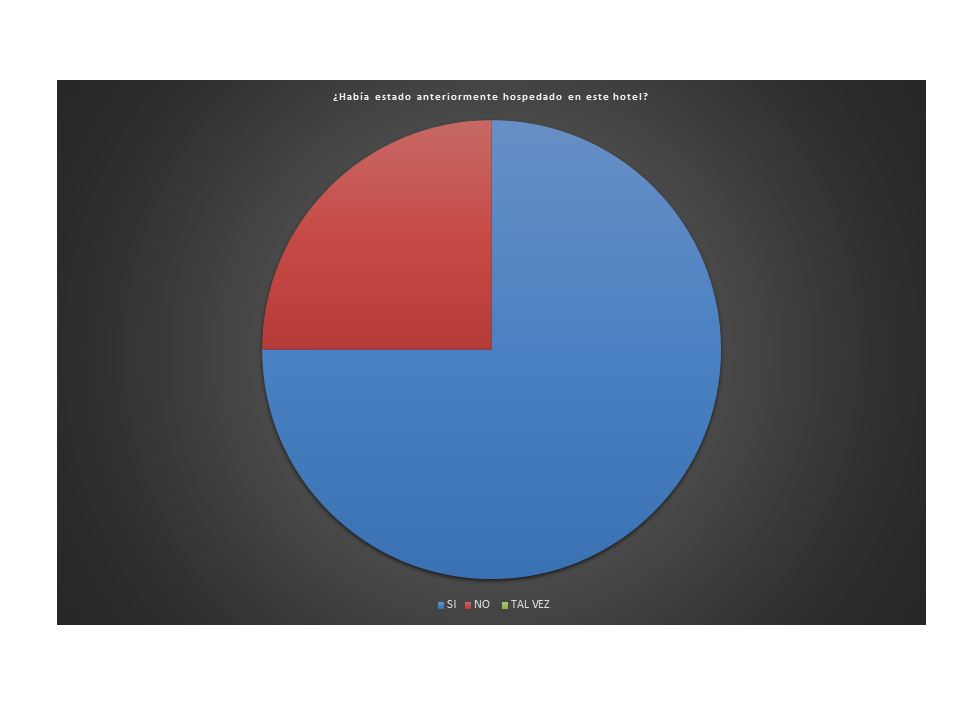
\includegraphics[scale=.7]{imagenes/Diapositiva1.PNG}
\caption{En la figura 1 puede ver que mas de la mitad de los clientes que recurre al hotel son clientes }
\end{figure}

\begin{figure}[H]
\centering
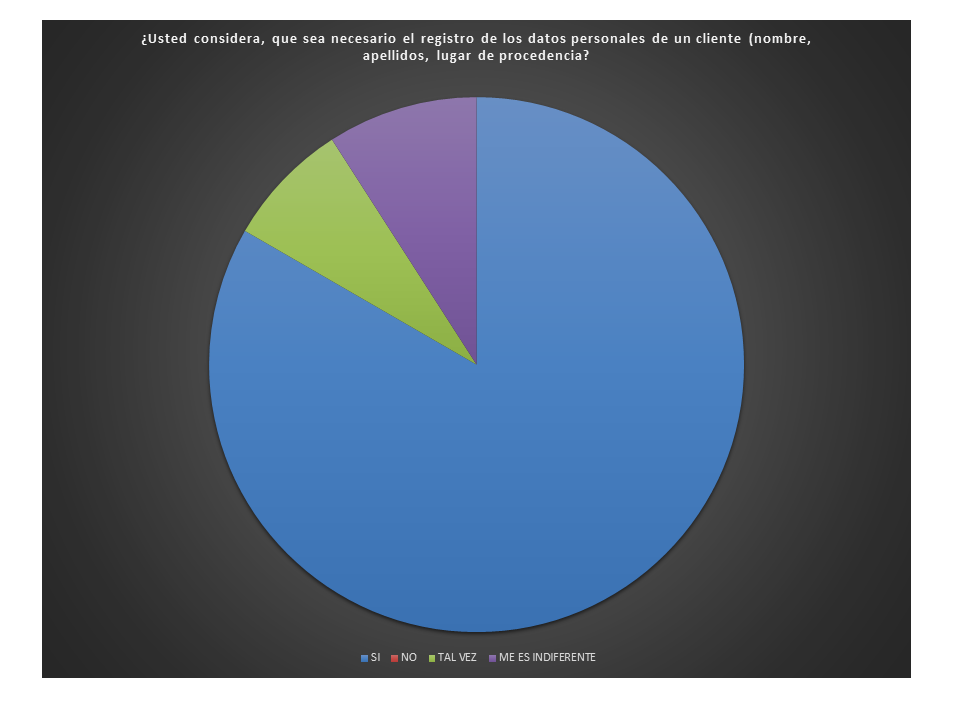
\includegraphics[scale=.7]{imagenes/Diapositiva2.PNG}
\caption{En la figura 2, se representa la opinion de los clientes del metodo de registro. }
\end{figure}


\begin{figure}[H]
\centering
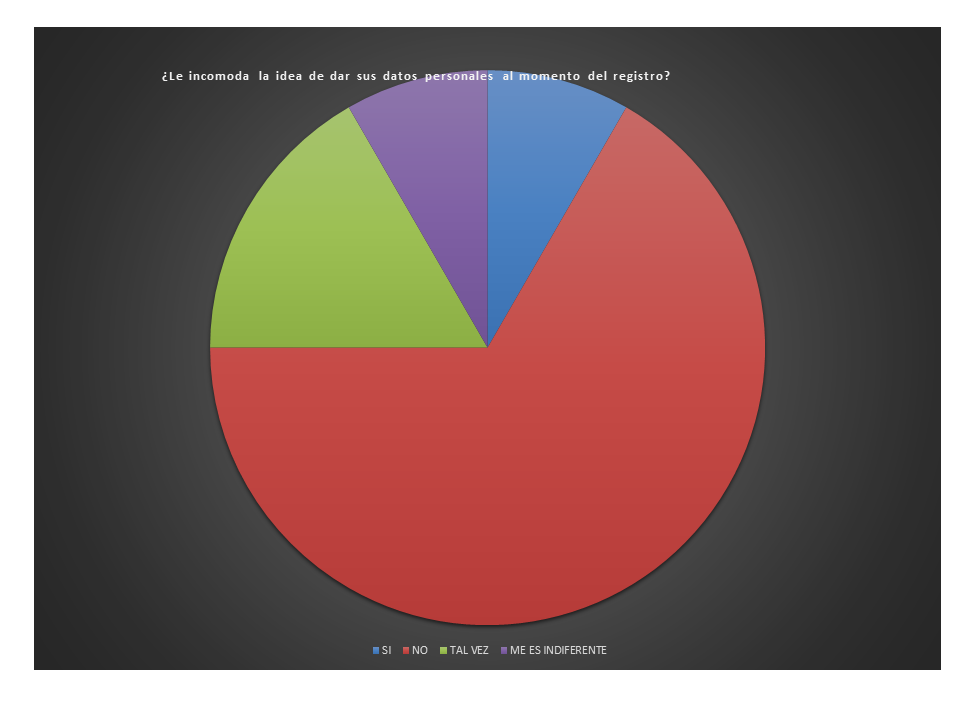
\includegraphics[scale=.7]{imagenes/Diapositiva3.PNG}
\caption{En la figura 3,se representa la disposición de los clientes de aportar sus datos para un registro al momento de ingresar al hotel.}
\end{figure}

\begin{figure}[H]
\centering
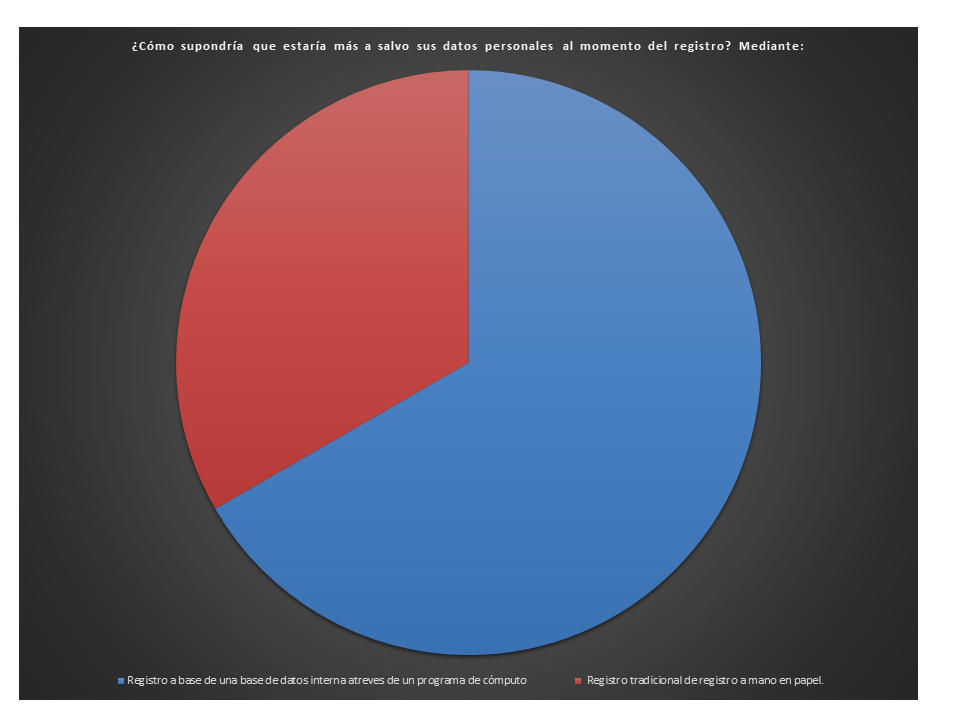
\includegraphics[scale=.7]{imagenes/Diapositiva4.PNG}
\caption{En la figura, se demuestra que los clientes optán por tomar un registro atravez de un sistema de computo que al registro a papel. }
\end{figure}' 

\begin{figure}[H]
\centering
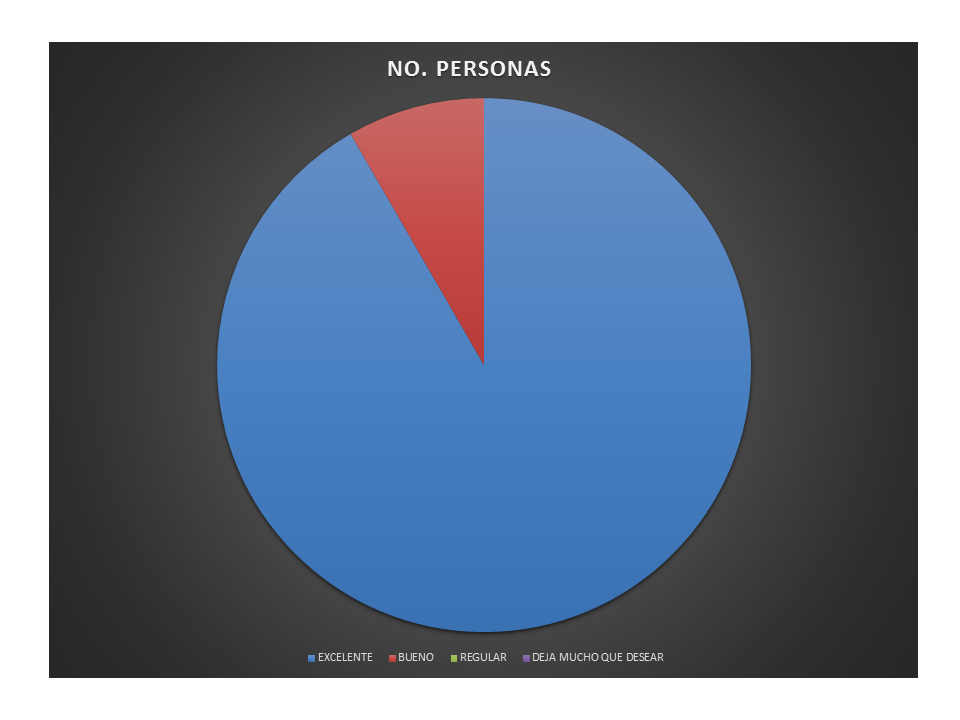
\includegraphics[scale=.7]{imagenes/Diapositiva5.PNG}
\caption{En la figura, en esta actividad se califica la atencion que considera que le ofrecio el recepcionista. }
\end{figure}

\begin{figure}[H]
\centering
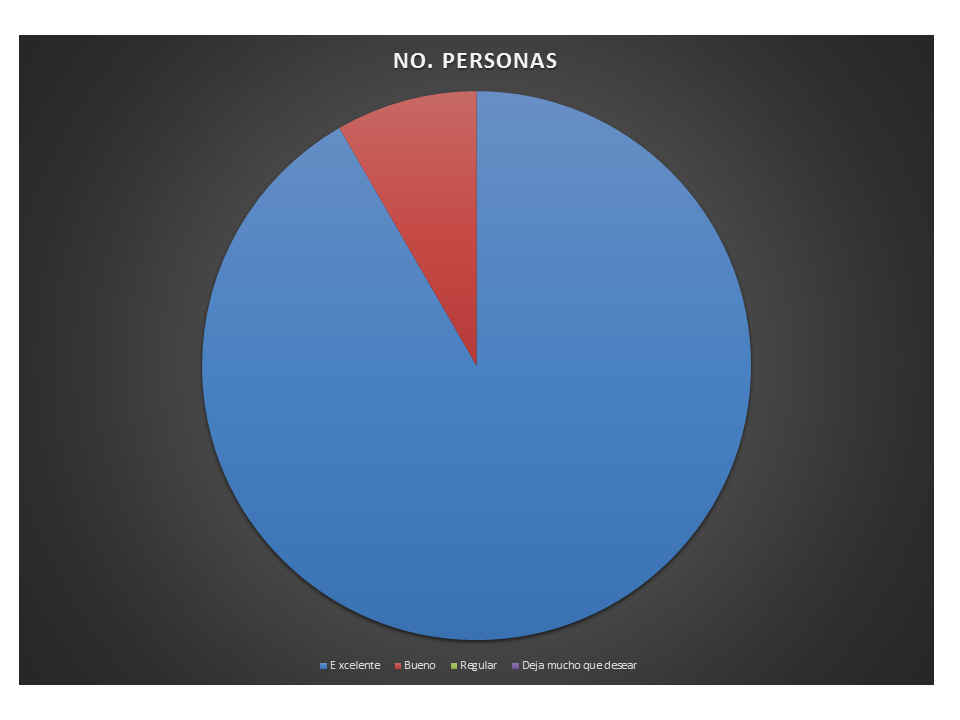
\includegraphics[scale=.7]{imagenes/Diapositiva6.PNG}
\caption{En la figura, se califico conforme a un porcentaje de clientes que fue registrada a travez del software. }
\end{figure}

\begin{figure}[H]
\centering
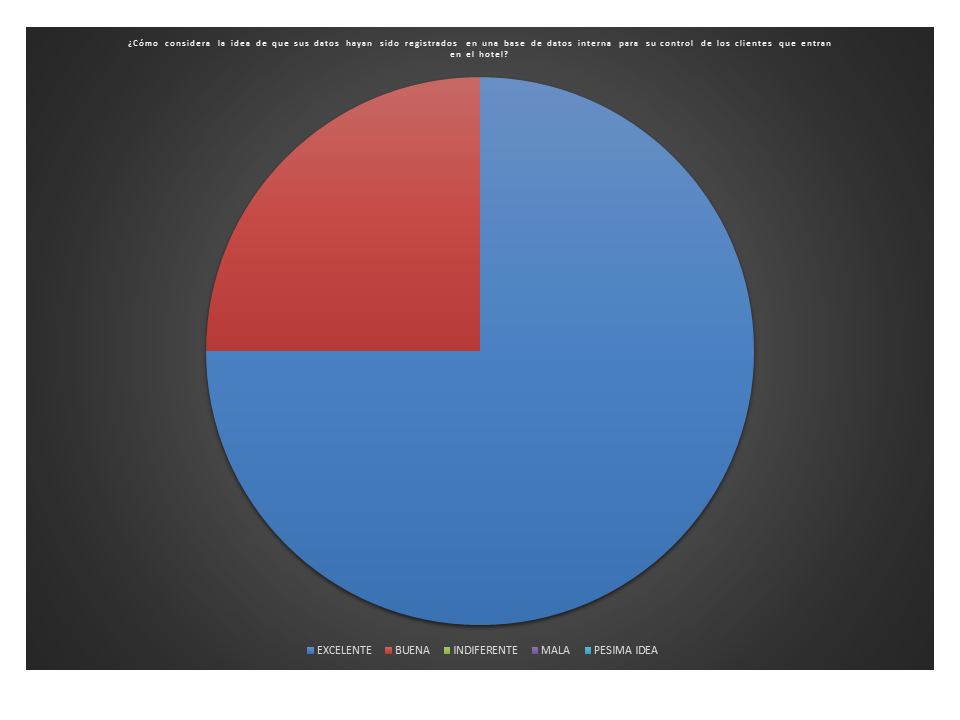
\includegraphics[scale=.7]{imagenes/Diapositiva7.PNG}
\caption{En la figura, se demuestra la opinión del cliente conforme a su registro. }
\end{figure}

\begin{figure}[H]
\centering
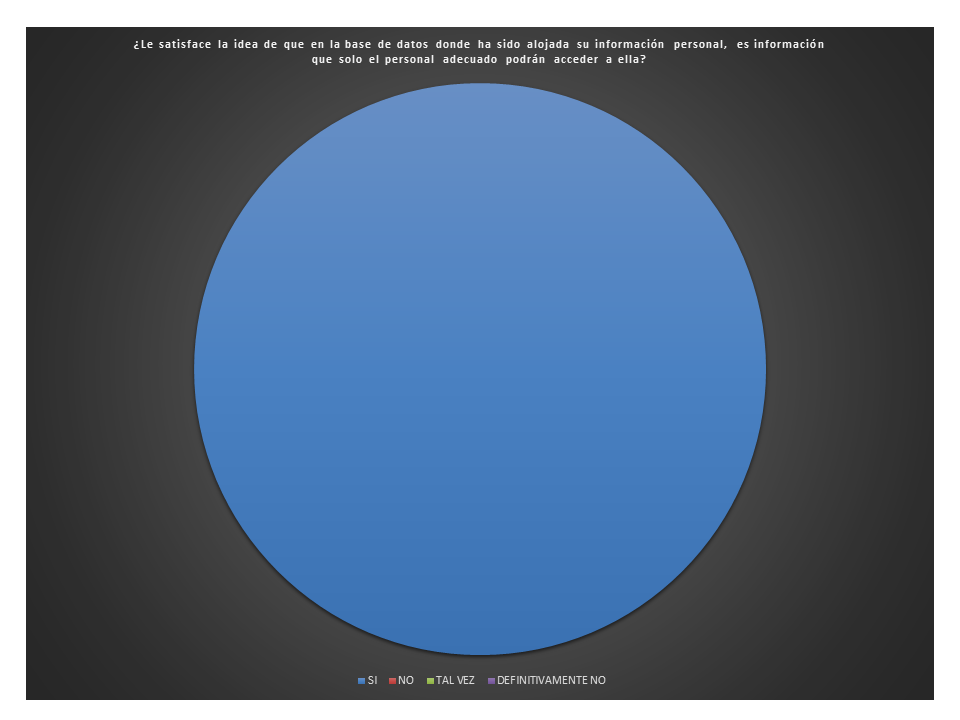
\includegraphics[scale=.7]{imagenes/Diapositiva8.PNG}
\caption{En la figura, se muestra la aceptación del cliente y conformidad en su registro a la entrada del hotel. }
\end{figure}

\begin{figure}[H]
\centering
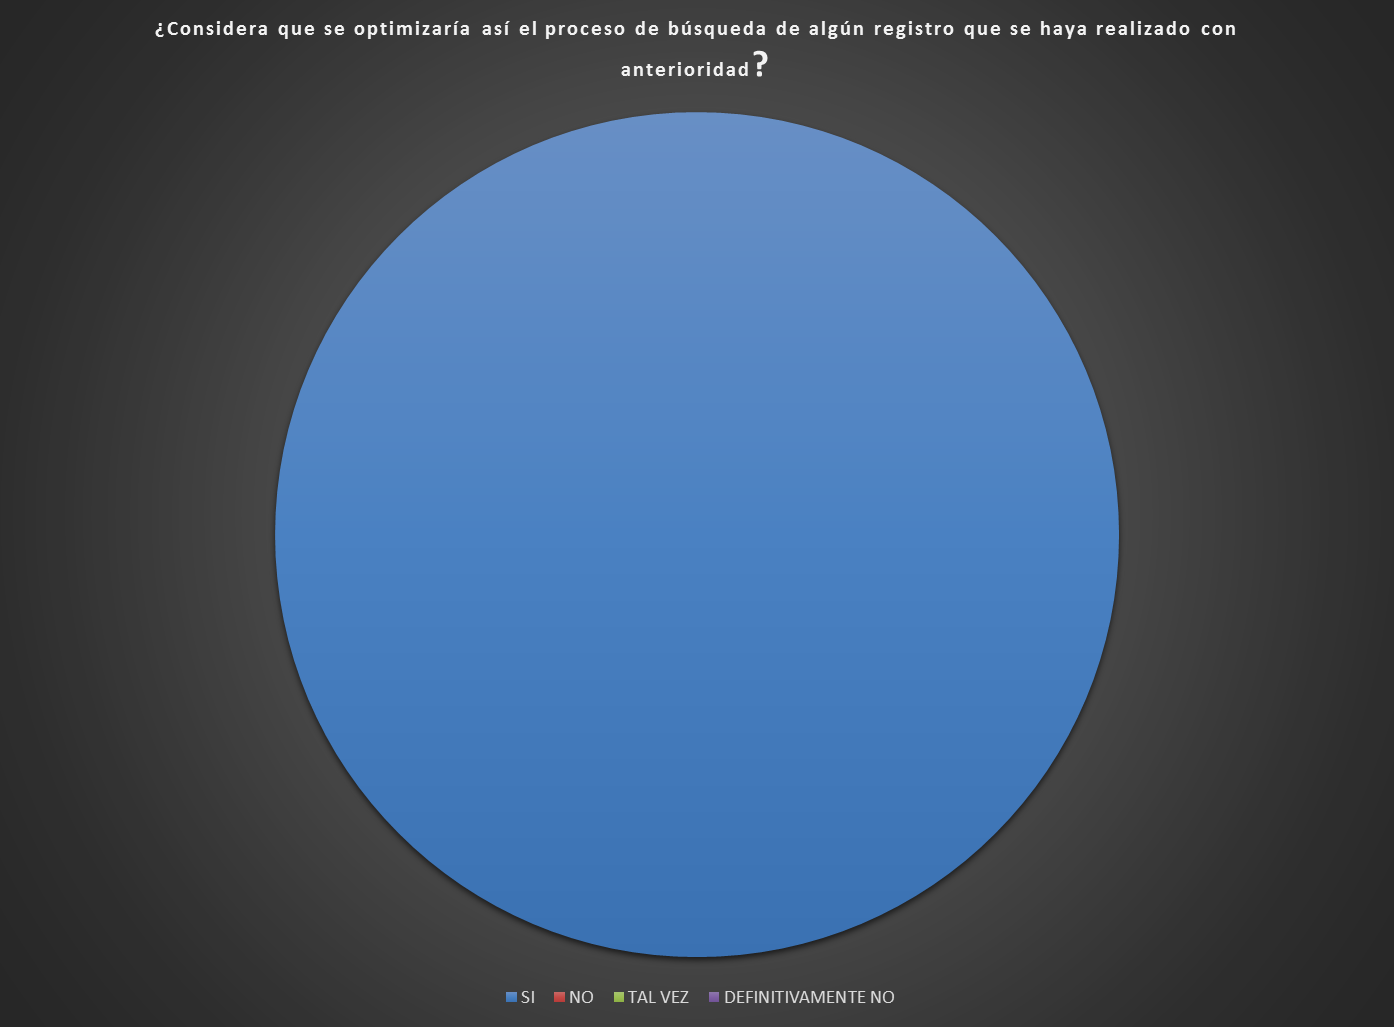
\includegraphics[scale=.7]{imagenes/Diapositiva9.png}
\caption{En la figura, los clientes demuestran su opinión conforme al registro que obtuvierón. }
\end{figure}

\end{document}



